\section{Protocolli di Trasporto}
I protocolli di trasporto sono un insieme di protocolli che risiedono sugli host e sugli endsystems; si occupano di fornire le regole per una comunicazione logica tra due entità remote.\\
A livello di invio, si occupano della ricezione dei messaggi in segmenti e li inviano al network layer; alla ricezione, i segmenti sono riassemblati in messaggi e passati al livello applicativo.\\
Mentre il livello di rete offre comunicazione tra due endsystems (trasportando informazioni da un host all'altro), il livello di trasporto crea un collegamento logico tra due \textit{processi}. Deve quindi essere in grado di raccogliere flussi informativi, utilizzare il livello di rete per trasportarli e successivamente smistarli nei vari processi applicativi.

\section{Internet transport-layer protocols}
A dispetto del fatto che il livello rete utilizza una best-effort policy che non dà nessuna garanzia di consegna, \textbf{TCP} si occuperà di applicare meccanismi per la traduzione di informazioni agli opportuni processi anche nel caso di perdita di dati.\\
I principali tipi di perdita dei dati sono:
\begin{itemize}
	\item un eccesso di informazioni arrivate al router intermedio. \\
	La conseguenza è un riempimento delle code fino al raggiungimento di una congestione in rete e all'inizio di una perdita di pacchetti.
	\item il ricevimento a destinazione di un tasso di informazioni troppo elevato rispetto alla velocità di lettura. \\
\end{itemize}
Si noti che un controllo del flusso di informazioni richiede algoritmi diversi rispetto al controllo di congestione; entrambi i tipi di controllo sono implementati da TCP.

\section{Multiplexing e Demultiplexing}
L'invio di informazioni da parte di un processo è eseguito attraverso una determinata porta dotata di interfacce ben definite. Tale porta, che consente il colloqui con l'entità sottostante di livello trasporto, prende il nome di \textit{socket}.\\
Poiché più flussi informativi sono trasmessi tramite lo stesso canale logico, occorre stabilire delle funzioni di smistamento di dati. Queste funzioni sono implementate nei protocolli TCP e UDP in maniera differente.\\

\subsection{UDP: Connectionless demux}
Il socket creato è dotato di un numero di porta dell'host locale; quando viene creato un \textit{datagram} (pacchetto) da inviare nel socket UDP, questo deve specificare l'indirizzo IP e il numero di porta dell'host di destinazione.
Quando l'host remoto riceve un segmento via UDP, controlla il suo numero di porta di destinazione e lo indirizza alla porta corrispondente.
Pacchetti con stesso numero di porta di destinazione, ma indirizzi IP o porte di origine differenti saranno quindi orientati allo stesso socket a destinazione.

\section{TCP: Connection-oriented demux}
In questo caso viene creato un socket dedicato al flusso di informazioni identificato dalla presenza di quattro campi: due per gli indirizzi IP del mittente e del destinatario, due per i numeri di porta del mittente e del destinatario.
Nel caso di più client connessi allo stesso webserver, all'inizio viene fatta una richiesta su un \textit{welcome-socket} generale; successivamente le richieste sono smistate ad un socket dedicato su ciascuna delle connessioni: in questo modo è assicurato che il flusso di dati passerà per socket differenti.
\newpage

\section{Reliable Data Transfer}
La necessità di strutturare un protocollo di trasferimento di dati affidabile nasce dall'importanza che due entità, in comunicazione, siano in equilibrio in termini di velocità di produzione/trasmissione/consumo dei dati, senza che l'eventuale fallimento nella trasmissione tramite livelli inferiori - nella pila TCP/IP - causi il definitivo fallimento della trasmissione. \\
Sarà fatto uso della rappresentazione FSM, una tipologia di rappresentazione utile alla sintetizzazione grafica dei servizi orientati alla connessione.
\begin{center}
    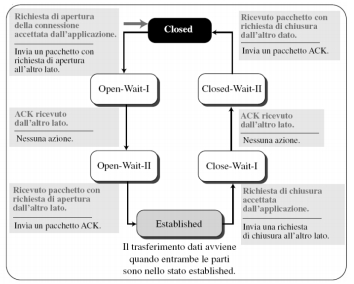
\includegraphics[width=.7\textwidth]{res/fsm.jpg} \hfill
\end{center}

\subsection{RDT 1.0}
Il caso riguardante \textit{RDT 1.0} è contestualizzato in una situazione perfettamente affidabile:
\begin{itemize}
    \item non si verificano \textbf{mai} errori nei bit trasmessi;
    \item non si verifica \textbf{mai} una perdita di pacchetti.
\end{itemize}
\begin{center}
    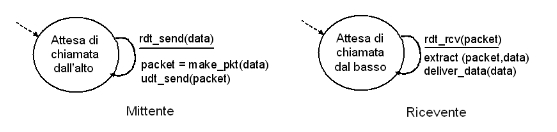
\includegraphics[width=.7\textwidth]{res/fsm-rdt-10.jpg} \hfill
\end{center}
\newpage

\subsection{RDT 2.0}
In questo caso, il canale di trasmissione effettiva può confondere i bit nel pacchetto. Da qui la necessità di introdurre dei messaggi di risposta alla ricezione di un pacchetto:
\begin{itemize}
    \item \textbf{ACK} (\textit{ACKnowledgment}, o \textit{conferma di ricezione}): utilizzato per confermare che il pacchetto è stato ricevuto ed è integro;
    \item \textbf{NAK} (\textit{Negative AcKnowledgment}, o \textit{conferma negativa}): il pacchetto contiene errori. Il mittente reinvia il pacchetto quando riceve indietro questo tipo di messaggio: motivo per cui si tratta di un protocollo \textit{ARQ} (\textit{Automatic Repeat reQuest}, o \textit{Richiesta Automatica di Ripetizione}.
\end{itemize}
\begin{center}
    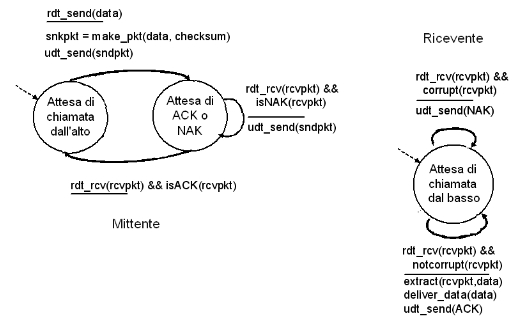
\includegraphics[width=.7\textwidth]{res/fsm-rdt-20.jpg} \hfill
\end{center}
\textit{RDT 2.0} può però andare incontro ad un difetto fatale: la mancata gestione degli eventi in cui i pacchetti \textit{ACK}/\textit{NAK} siano danneggiati.

\subsection{RDT 2.1}
Viene dunque aggiunto - alternativamente - un valore binario a ciascun pacchetto, un \textit{numero di sequenza}.
In questo modo, viene comunicato non solo l'esito della ricezione al mittente, ma anche il pacchetto a cui questo fa riferimento. \\
\begin{minipage}[t]{0.5\textwidth}
    \begin{center}
        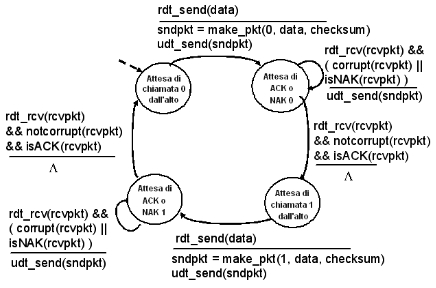
\includegraphics[width=.8\textwidth]{res/fsm-rdt-21-sender.jpg} \hfill
    \end{center}
\end{minipage}
\begin{minipage}[t]{0.5\textwidth}
    \begin{center}
        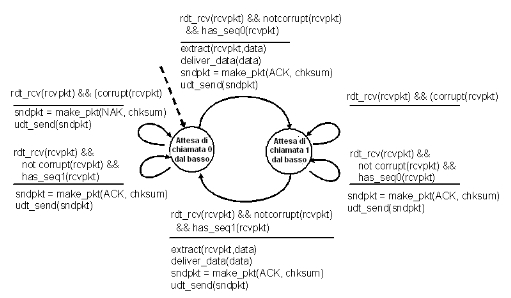
\includegraphics[width=.8\textwidth]{res/fsm-rdt-21-receiver.jpg} \hfill
    \end{center}
\end{minipage}
\newpage

\subsection{RDT 2.2}
\textit{RDT 2.2} fornisce le stesse funzionalità di \textit{RDT 2.1}, utilizzando però soltanto gli \textit{ACK}, escludendo i \textit{NAK}.
Nel caso in cui il destinatario dovesse inviare un \textit{NAK}, invia nuovamente un \textit{ACK} con numero di sequenza dell'ultimo pacchetto ricevuto correttamente.
\begin{center}
    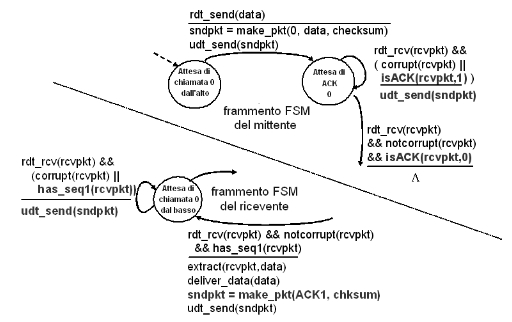
\includegraphics[width=.7\textwidth]{res/fsm-rdt-22.jpg} \hfill
\end{center}

\subsection{RDT 3.0}
L'alternativa è invece introdurre una nuova funzione di timing. Per ogni pacchetto inviato, il mittente implementa un timer: una volta che questo raggiunge un timeout, se non ha ricevuto nessun pacchetto che gli comunichi l'esito (l'\textit{ACK}), allora reinvia il pacchetto. Per questo motivo:
\begin{itemize}
    \item il mittente deve tenere una copia del pacchetto spedito fino a che non ne riceve riscontro dell'esito;
    \item per garantire il controllo di flusso, non si spedisce più di un pacchetto alla volta.
\end{itemize}
Il parametro \textit{RTT} (o \textit{Round Trip Time}) viene definito come il tempo necessario per l'invio di un pacchetto sommato a quello per la ricezione di un pacchetto riferito all'esito del precedente.
\paragraph{Esempio.}
In un link da 1Gbps, con un \textit{propagation delay} di 15ms e 8000bit per ciascun pacchetto abbiamo:
\begin{center}
$ D = \frac{L}{R} = \frac{8000bit}{10^9 bit/s} = 8microsecs $ \\
$ U = \frac{\frac{L}{R}}{RTT + \frac{L}{R}} = \frac{0,0008}{30,0008} = 0,00027 $
\end{center}
\newpage

\subsection{Protocolli a Ritrasmissione Automatica (o \textit{a finetra})}
A differenza dei precedenti, viene trasmessa sempre una sequenza di pacchetti. A man mano che si ricevono gli ACK, vengono aggiunti nuovi pacchtti in coda.
In questo caso: $ U = \frac{\frac{3L}{R}}{RTT + \frac{L}{R}} $ \\
\paragraph{Go-back-N.} Il mittente può avere fino a N pacchetti non riconosciuti nella pipeline. Il destinatario invia solo \textit{ACK cumulativi}, ovvero relativi ad un gruppo di pacchetti ricevuti. Il mittente utilizza un timer per legato al primo pacchetto inviato che ancora non ha ricevuto ACK: al suo raggiungimento, reinvia tutti i pacchetti a partire da quello per il quale ha impostato il timeout.
\paragraph{Selective Repeat.} Il mittente può avere fino a N pacchetti. Il destinatario invia un \textit{ACK individuae}, relativo quindi ad ogni pacchetto. Il mittente utilizza invece un timer per ogni pacchetto di cui non ha ricevuto esito; quando raggiunge il timeout, ritrasmette solo quel dato pacchetto.

\section{Ritrasmissione Automatica in TCP}
TCP utilizza una versione ibrida dei protocolli \textit{Go-back-N} e \textit{Selective repeat}: invia un flusso di singoli bytes che formano - per mano del ricevente - un segmento, il cui \textit{sequence number} è quello del primo byte contenuto, e la cui lunghezza è determinata dal numero totale di bytes. Utilizza inoltre una variabile definita come \textit{MSS}, che indica la lunghezza massima di ciascun segmento. \\
In una stessa connessione, il flusso di dati è bidirezionale, viene eseguito un \textit{handshake} per inizializzare i buffer e alcune variabili (come la \textit{MSS} stessa). La dimensione dei buffer varia nel tempo, sulla base delle informazioni raccolte dai controlli di flusso e congestione. \\
Ogni segmento è composto dai seguenti campi (ciascuno da 32bit):
\begin{itemize}
	\item Porta sorgente / destinazione;
	\item \textit{Sequence number};
	\item \textit{Acknowledgment number}: eventuale ACK di riscontro per un pacchetto appena ricevuto (necessario perché la connessione è bidirezionale);
	\item \textit{Checksum};
	\item \textit{Header length}: se si desidera aggiungere informazioni addizionali, è necessario specificarne la lunghezza;
	\item \textit{Receive window}: indica quanto spazio ho ancora nel buffer (necessario per la gestione del flusso);
	\item \textit{RST}/\textit{SYN}/\textit{PIN}: variabili settate a \textit{1} in fase di apertura/chiusura della connessione;
	\item \textit{ACK}: variabile settata a \textit{1} se il ricevente deve leggere il campo \textit{Acknowledgment number};
	\item \textit{URG}: indica che si tratta di un pacchetto più urgente della media;
	\item \textit{Application Data}: dati da trasmettere.
\end{itemize}

\subsection{Meccanismi di controllo affidabile}
In \textit{TCP} - lato \textit{sender} - viene, per ciascuna connessione e trasmissione, creato un segmento con \textit{numero di sequenza} \textit{n}, che corrisponde al primo byte del flusso di bytes in trasmissione attraverso quello stesso segmento. \\
Se un timer è già attivo, rimane invariato, perché ancora non è stato ricevuto riscontro su una serie di segmenti; altrimenti, lo avvio. \\
Al timeout, ritrasmesso il primo segmento che lo ha causato, ma non tutto, perché \textit{TCP} permette l'inserimento dei buffer contenenti i flussi di bytes ricevuti non necessariamente in sequenza per conservarli. Poi viene riavviato il timer. \\
Al ricevimento dell'\textit{ACK}, si controlla se è relativo ad un segmento di cui non si conosce l'esito di ricezione:
\begin{enumerate}
    \item applico l'\textit{ACK} a tutti i segmenti di cui non avevo ancora ricevuto l'esito fino a quest'ultima ricezione;
    \item avvio un nuovo timer.
\end{enumerate}

\subsection{Variabilità del retransmission timeout}
Ovviamente, il timeout deve essere necessariamente $/geq RTT$ (\textit{RoundTrip Time}). Inoltre:
\begin{itemize}
    \item se troppo corto, avvengono ritrasmissioni inutili e non necessarie;
    \item se troppo lungo, i tempi di reazione diventano troppo lunghi se i segmenti sono andati perduti.
\end{itemize}
Per ovviare a questi problemi, è stato introdotto una stima calcolata per ottenere dinamicamente un timeout più adatto alle prestazioni di rete di ciascuna connessione. Viene utilizzato un \textit{SampleRTT}, ovvero l'\textit{RTT} dell'ultima trasmissione eseguita della quale è stato ricevuto l'\textit{ACK}. A questo punto viene utilizzata una media esponenziale pesata per tenere in conto della variabilità nel tempo dei vari \textit{SampleRTT}, nella cui formula viene utilizzata una variabile $\alpha$, tipicamente impostata a \textit{0,125}, la cui funzione è quella di dare maggiore importanza ai \textit{SampleRTT} più recenti, rispetto che a quelli più lontani nel tempo. Il risultato è la seguente formula: \\
\begin{center}
    $ EstimatedRTT = (1-\alpha )\times EstimatedRTT + \alpha \times SampleRTT $
\end{center}
A questo punto, questa stima viene utilizzata nel calcolo della deviazione dell'\textit{RTT}, in cui compare una nuova variabile $\beta$, la cui funzione è identica a quella della variabile $\alpha$ vista in precedenza, ma che è tipicamente valutata \textit{0,25}: \\
\begin{center}
    $ DevRTT = (1-\beta )\times DevRTT + \beta \times \left| SampleRTT - EstimatedRTT \right| $
\end{center}
Infine, il valore del timeout stimato come migliore possibile ed effettivamente utilizzato:
\begin{center}
    $ Timeout = EstimatedRTT + 4 \times DevRTT $ \\
\end{center}

\subsection{Controllo del flusso}
Il \textit{Flow Control} è utilizzato per evitare di saturare il \textit{buffer} dentro cui vengono conservati i pacchetti ricevuti, prima che vengano prelevati dal \textit{layer applicativo}. Se questo venisse riempito troppo rapidamente, rispetto alla velocità di prelevamento dei dati, ci si troverebbe in una situazione di criticità. \\
Per questa ragione, vengono segnalate al \textit{sender} informazioni sullo spazio a disposizione, nel campo \textit{receive window} (da \textit{16bit}) nel segmento: il \textit{sender} adegua il flusso dei dati trasmesso di conseguenza. \\
La \textit{finestra} e il \textit{buffer} sono configurati nell'\textit{handshake} della connessione, tramite i campi:
\begin{itemize}
    \item \textbf{MSS} (\textit{Maximum Sequence Size}): impostato tipicamente a 2K, indica la lunghezza massima del segmento;
    \item \textbf{ISN} (\textit{Initial Sequence Number)}: impostato tipicamente a 2047 (e chiaramente variando in base al valore del \textit{MSS}), indica il valore iniziale del \textit{sequence number};
    \item \textbf{WIN} (\textit{WINdow}): impostato tipicamente a 4K, indica la dimensione della finestra.
\end{itemize}
Ad ogni trasmissione, viene specificato anche il valore \textit{WIN} sulla base dello spazio rimanente disponibile sul \textit{buffer} del ricevitore. \\
Potrebbe però accadere che il segmento di notifica da parte del ricevitore che lo spazio sul \textit{buffer} è tornato disponibile vada perduta. Per questa ragione, il \textit{sender} continua \textit{sempre} ad inviare pacchetti - piccoli, se il \textit{buffer} è stato segnalato come saturo -, a distanza di timeout crescenti nel tempo (possono raggiungere massimo 60s), così da rimanere in contatto con il ricevitore e poter sapere se il \textit{buffer} contiene nuovamente spazio a sufficienza per ricevere dati utili.